%%% Pakete %%%
\documentclass[11pt,landscape]{beamer}
%\documentclass[11pt,landscape,notes]{beamer}
%\documentclass[11pt,handout,notes=only]{beamer}
\usepackage{tikz} 
\usetikzlibrary{shapes,shapes.geometric,arrows,fit,calc,positioning,automata,backgrounds,arrows.meta}

\tikzstyle{decision} = [diamond, draw, fill=yellow!20, text width=4.8em, text badly centered, inner sep=0pt]
\tikzstyle{timer} = [circle, draw, fill=orange!20, text width=4.8em, text badly centered, inner sep=0pt]
\tikzstyle{block} = [rectangle, draw, fill=blue!20, text width=5.7em, text centered, rounded corners, minimum height=3em]
\tikzstyle{line} = [draw, -latex']
\tikzstyle{start} = [draw, ellipse,fill=green!20, text width=4.8em, text centered, node distance=3cm, minimum height=1em]
\tikzstyle{stop} = [draw, ellipse,fill=red!20, node distance=3cm, minimum height=1em]
%\DeclareMathSizes{11}{30}{15}{10}
%\DeclareMathSizes{13}{30}{15}{10}
%\DeclareMathSizes{10}{30}{15}{10}
\usepackage{tipa}
\usepackage[T1]{fontenc}
\usepackage{interval}
\usepackage{lmodern}
\usepackage[utf8]{inputenc}
\usepackage{german}
\usepackage{ragged2e}
\usepackage{epstopdf}
\usepackage{bbding}
\usepackage{amsmath}
\usepackage{relsize}
\usepackage{xfrac}
\usepackage{listings}
\usepackage{color}
\usepackage{expl3}[2015/03/01]
\usepackage{media9}[2015/03/01]
\usepackage{multimedia}
\usepackage{graphicx}
\usepackage{eurosym}
\mode<presentation>{\usetheme{E2}}
\setbeamertemplate{navigation symbols}{}
\newcommand{\lc}[1]{\texttt{\textbackslash#1}}
\newcommand{\lcp}[2]{\texttt{\textbackslash#1\{#2\}}}
\newcommand{\lco}[2]{\texttt{\textbackslash#1[#2]}}
\newcommand{\lcop}[3]{\texttt{\textbackslash#1[#2]\{#3\}}}
\newcommand{\lcpp}[3]{\texttt{\textbackslash#1\{{#2}\}\{{#3}\}}}
\newcommand{\lcppp}[4]{\texttt{\textbackslash#1\{#2\}\{#3\}\{#4\}}}
\newcommand{\lcopp}[4]{\texttt{\textbackslash#1[#2]\{#3\}\{#4\}}}
\newcommand{\lenv}[2]{\texttt{\textbackslash{}begin\{#1\}\linebreak[0]#2\linebreak[0]\textbackslash{}end\{#1\}}}
\newcommand{\todo}[2]{\colorbox{orange}{\textbf{#1:} {#2}}}
\newcommand{\ds}{\ensuremath\displaystyle}
\newenvironment{determinante}[1]{%
\ensuremath\left|\begin{array}{#1}}{%
\end{array}\right|}
\AtBeginSection[]
{
 \begin{frame}<beamer>
 \frametitle{\"Ubersicht}
 \tableofcontents[currentsection]
 \end{frame}
}
%\AtBeginSubsection[]
%{
% \begin{frame}<beamer>
% \frametitle{\"Ubersicht}
% \tableofcontents[currentsection, currentsubsection]
% \end{frame}
%}
\definecolor{lightgray}{gray}{.9} 
\definecolor{noalpha}{gray}{1} 

%%% Daten %%%

\title{Energieeffizientes Routing in Ad-Hoc Netzen}
\subtitle{Eine simulationsbasierte Analyse von AODV und OLSR}
\author{Marcel Ebbrecht} 
\institute{TU Dortmund, Bachelorabschlussvortrag}
\date{\today}
\makeindex

%%% Beginn Dokument %%%

\begin{document}
\setlength{\parskip}{1mm}

%%% Titelseite %%%
\begin{frame}[c,label=titlepage]
  \titlepage
\end{frame}

\logo{}
%\begin{frame}[t, label=overview]
%  \frametitle{\"Ubersicht}
  \setcounter{tocdepth}{1}
%  \tableofcontents
%\end{frame}

%%% Teil 1 - Vorarbeit %%%

\section{Vorarbeit}

\subsection{Whoami}

\begin{frame}{\insertsubsection}
\begin{itemize}
\item Marcel Ebbrecht\newline
\item Viele Jahre LAN, WAN, WLAN, TCP/IP\newline
\item $n$ Jahre Informatik\newline
\item marcel.ebbrecht@googlemail.com\newline
\item https://github.com/marcelebbrecht/powerrouting
\end{itemize}
\end{frame}

\note[itemize]{
\item Bla
\item Bla
\item Geht nur mich und Prüfungsamt was an
\item Bei Fragen, etc.
\item Software, Thesis und Präsentation wenn durch, Commit an INETMANET
}

%\subsection{Vorbemerkungen}

%\begin{frame}{\insertsubsection}
%\begin{itemize}
%\item Live-On-Tape\newline
%\item Real ist cooler, Simulation einfacher\newline
%\item Routing ist wichtig\newline
%\item MESH wird es
%\end{itemize}
%\end{frame}

%\note[itemize]{
%\item Aufgenommen, Notebook lahm, Vorspulen -> Spart Zeit, Omnet GUI-Simulator zickig\newline
%\item Keine Geräte und Messtechnik, vollkommen kontrollierte Bedingungen, nur Teile der Realität die wir brauchen, hat aber auch Tücken (später)\newline
%\item Riesen Netze weltweit, Routing verbindet uns\newline
%\item Steigender Bedarf an Bandbreite, Hochverfügbarkeit, politische Gründe, Infrastruktur schaffen (WSAN, billige Infrastruktur (OLPC in Schwellenländern)), unreguliert und unabhängig (Freifunk OLSR oder PacketRadio)
%}

%\subsection{Worum geht es nicht?}

%\begin{frame}{\insertsubsection}
%\begin{itemize}
%\item TCP/IP\newline
%\item Routing\newline
%\item WLAN
%\end{itemize}
%\end{frame}

%\note[itemize]{
%\item Keine Grundlagen in TCP/IP -> IP Adressen, Subnetting sollte bekannt sein%\newline
%\item Keine Grundlagen in Routing -> Routingtabelle, Router sollte bekannt sein\newline
%\item Keine Grundlagen in WLAN -> Ad-Hoc sollte bekannt sein
%}

\subsection{Warum sind wir hier?}

\begin{frame}{\insertsubsection}
\begin{itemize}
\item Was ist das Problem und warum ist das relevant?\newline
\item OLSR und AODV im Wesentlichen\newline
\item Optimierung nach Ladezustand\newline
\item Nach dem Vortrag gerne mehr Videos und Auswertungen
\end{itemize}
\end{frame}

\note[itemize]{
\item Problem wird beschrieben, Relevanz erläutert\newline
\item Grundeigenschaften und Funktionen, die für das Verständnis der Anpassung wichtig sind\newline
\item Die eigentliche Arbeit, Videos, Auswertungen, Vergleiche, Fazit\newline
\item Sehr viel vorhanden, im Vortrag größtenteils AODV, ist zwar nicht so sauber implementiert wie OLSR, aber in Videos schneller erkennbar
}

\begin{frame}{\insertsubsection}
  \begin{center}
\includegraphics[scale=0.45]{aodv-unstable}
  \end{center}
\end{frame}

\subsection{Something completely different}

\begin{frame}{\insertsubsection}
\begin{center}
\Huge{\textbf{\textipa{[\textprimstress ra\textsubarch{\textupsilon}t\textschwa (r)]}}}
\end{center}
\end{frame}

\note[itemize]{
\item Immer wieder Diskussionen ... 
}

\subsection{Rauter}

\begin{frame}{\insertsubsection}
\includegraphics[scale=0.50]{rauter} \newline
\tiny{Quelle: https://www.stern.de}
\end{frame}

\note[itemize]{
\item Ein männlicher Rauter
}

\subsection{Zentrale Erkenntnis vorweg}

\begin{frame}{\insertsubsection}
\begin{center}
\Huge{\textbf{\textipa{[\textprimstress ru:t\textschwa (r)]}}}
\end{center}
\end{frame}

\note[itemize]{
\item Eine wirklich sinnvolle Sache möchte ich noch vermitteln\newline
\item Immer wieder Kollegen getroffen, die Rauter sagen\newline
\item Die Engländer haben es von den Franzosen, die sagen route mit u
}

\subsection{Ruuuuuter}

\begin{frame}{\insertsubsection}
\includegraphics[scale=0.15]{router} \newline
\tiny{Quelle: https://www.pcwelt.de}
\end{frame}

\note[itemize]{
\item Wir meinen im weitesten Sinne solche Geräte\newline
\item Kann aber alles sein, was im Netzwerk Nachrichten zwischen Segmenten vermitteln kann: Smartphones, Sensoren, PCs, Notebooks, etc.
}

%%% Teil 2 - Routing %%%

\section{Routing}

\subsection{Allgemein}

\begin{frame}{\insertsubsection}
\begin{itemize}
\item TCP/IP Layer 3\newline
\item IPv4 (IPv6)\newline
\item Statisches Routing\newline
\item Dynamisches Routing (reaktiv oder proaktiv)\newline
%\item Metriken
\end{itemize}
\end{frame}

\note[itemize]{
\item Vermittlung zwischen IP-Subnetzen\newline
\item Die Arbeit betrachtet IPv4, Aussagen gelten aber auch für IPv6, Protokolle können das\newline
\item Pflege von Routeninformationen (Ziel, Gateway, Metrik) per Hand, kleine statische Netze\newline
\item Bereitstellung über Routingprotokolle, wenn gebraucht oder permanent\newline
\item Die Güte einer Verbindung, i.d.R. kommt diese in der Routingtabelle des Systems als Zahl an, je kleiner, desto besser. Simple Metrik: HopCount (Anzahl der Knoten bis zum Ziel) oder differenzierter -> Das entscheiden die Routingprotokolle, gr. und/oder dyn. Netze
}

\subsection{Ad-hoc On-demand Distance Vector}

\begin{frame}{\insertsubsection}
\begin{itemize}
\item Reaktiv\newline
\item Geringer Overhead / Hohe Latenz\newline
\item Loop avoidance\newline
\item Precursors-Listen\newline
\item HopCount maßgebend
\end{itemize}
\end{frame}

\note[itemize]{
\item Fordert Routen an, wenn sie gebraucht werden (Name!!!)\newline
\item Hierdurch kein Traffic, wenn keine neuen Routen gebraucht werden, dafür aber Wartezeit beim Bedarf nach neuer Route\newline
\item Durch Sequenznummern wird das DV-Prot. typische Problem vermieden (im Prinzip werden nur Infos verarbeitet, die eine höhere Nummer haben)\newline
\item Speichert pro Route Informationen über Hosts, die diese Route nutzen\newline
\item HC einzig maßgebend für Routenwahl durch OS (!= Protokoll!!!)\newline
\item Gute Anwendung: Sensornetz - ein Ziel, wenig Overhead (Strom)
}

\subsection{AODV Ablauf}

\begin{frame}{\insertsubsection}
\begin{itemize}
\item Route benötigt -> RREQ\newline
\item Route bekannt -> RREP\newline
\item Route nicht mehr verfügbar -> RERR\newline
\item Sammelt Informationen aus empfangenen Nachrichten\newline
\item Entfernt Routen durch Timeout oder RERR
\end{itemize}
\end{frame}

\note[itemize]{
\item Versand per Broadcast, TTL wird schrittweise gesteigert bei Timeout\newline
\item Ein Host der eine Route kennt, schickt RREP per Unicast an den Originator des RREQ\newline
\item Stellt ein Router den Ausfall einer Route fest, ob durch Detektion oder RERR, wird er die Precursors dieser Routen informieren (Hier UC, BC geht auch), mehrere Ziele in einem RERR\newline
\item Gewinnt Routinginformationen aus AODV RREQ (Broadcast) und weitergeleiteten RREPs (Unicast) von Nachbarn, Refresh\newline
\item Nach gewisser Zeit verschwinden inaktive Routen
}

\subsection{Optimized Link State Routing}

\begin{frame}{\insertsubsection}
\begin{itemize}
\item Proaktiv\newline
\item OLSR Paket mit Messages\newline
\item MID, HELLO, TC\newline
\item 1HNB, 2HNB, MPRSet (\glqq optimized\grqq) \newline
\item Willingness
\end{itemize}
\end{frame}

\note[itemize]{
\item Name!!! Permanenter Austausch von Informationen, auch ohne Anforderung von Routen -> Overhead immer gegeben, dafür Routen nach Vorlaufzeit sofort verfügbar\newline
\item Mehrere Messages per Paket möglich -> spart Traffic\newline
\item Minimale zu unterstützende Menge ... zu aufwändig wie es genau funktioniert; MID/TC BC TTL255 Routenfindung, HELLO Sensing und MPRs mitteilen\newline
\item 1 direkte Nachbarn, 2 direkte Nachbarn von 1 ohne Host selbst, MPRSet minimale Menge an 1HNB um alle 2HNB zu erreichen (jeder Router eigenes Set, regelmäßige Neuberechnung)\newline
\item Bereitschaft zu Routen, 7 hoch, 1 minimum, relevant für Aufnahme ins MPRSet
}

\subsection{Ohne Willingness}

\begin{frame}{\insertsubsection}
  \begin{center}
  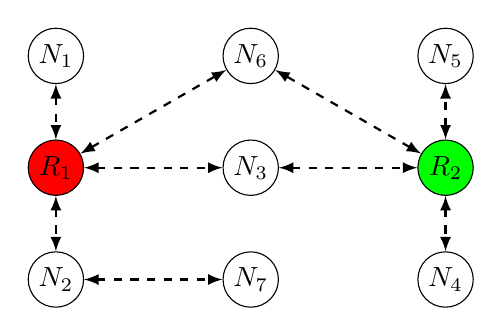
\begin{tikzpicture}[ 
    >=stealth',node distance=3cm, 
    node/.style={circle,minimum size=2.0em,draw}] 
    \node[label=center:$N_1$,node] (N1) [] {}; 
    \node[label=center:$R_1$,node,fill=red] (R1) [below=2em of N1] {}; 
    \node[label=center:$N_2$,node] (N2) [below=2em of R1] {}; 
    \node[label=center:$N_3$,node] (N3) [right=5em of R1] {}; 
    \node[label=center:$R_2$,node,fill=green] (R2) [right=5em of N3] {}; 
    \node[label=center:$N_4$,node] (N4) [below=2em of R2] {};
    \node[label=center:$N_5$,node] (N5) [above=2em of R2] {};
    \node[label=center:$N_6$,node] (N6) [above=2em of N3] {};
    \node[label=center:$N_7$,node] (N7) [below=2em of N3] {};

    \draw[>=latex,auto=right,style={<->},thick,dashed] (N1) -- (R1);
    \draw[>=latex,auto=right,style={<->},thick,dashed] (R1) -- (N2);
    \draw[>=latex,auto=right,style={<->},thick,dashed] (R1) -- (N3);
    \draw[>=latex,auto=right,style={<->},thick,dashed] (N3) -- (R2);
    \draw[>=latex,auto=right,style={<->},thick,dashed] (R2) -- (N4);
    \draw[>=latex,auto=right,style={<->},thick,dashed] (R2) -- (N5);
    \draw[>=latex,auto=right,style={<->},thick,dashed] (R1) -- (N6);
    \draw[>=latex,auto=right,style={<->},thick,dashed] (R2) -- (N6);
    \draw[>=latex,auto=right,style={<->},thick,dashed] (N2) -- (N7);
  \end{tikzpicture}
  \end{center}
  1HNB($R_1$) = \{$N_1,N_2,N_3,N_6$\} - 2HNB($R_1$) = \{$N_7,R_2$\}\newline
  1HNB($R_2$) = \{$N_3,N_4,N_5,N_6$\} - 2HNB($R_2$) = \{$R_1$\}
\end{frame}

\begin{frame}{\insertsubsection}
  \begin{center}
  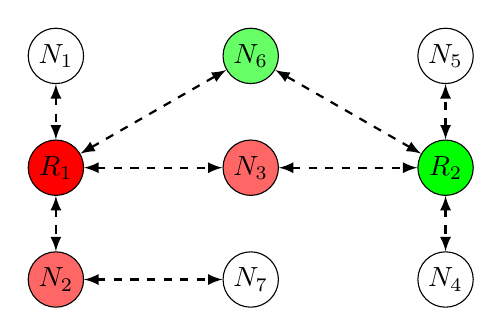
\begin{tikzpicture}[ 
    >=stealth',node distance=3cm, 
    node/.style={circle,minimum size=2.0em,draw}] 
    \node[label=center:$N_1$,node] (N1) [] {}; 
    \node[label=center:$R_1$,node,fill=red] (R1) [below=2em of N1] {}; 
    \node[label=center:$N_2$,node,fill=red!60] (N2) [below=2em of R1] {}; 
    \node[label=center:$N_3$,node,fill=red!60] (N3) [right=5em of R1] {}; 
    \node[label=center:$R_2$,node,fill=green] (R2) [right=5em of N3] {}; 
    \node[label=center:$N_4$,node] (N4) [below=2em of R2] {};
    \node[label=center:$N_5$,node] (N5) [above=2em of R2] {};
    \node[label=center:$N_6$,node,fill=green!60] (N6) [above=2em of N3] {};
    \node[label=center:$N_7$,node] (N7) [below=2em of N3] {};

    \draw[>=latex,auto=right,style={<->},thick,dashed] (N1) -- (R1);
    \draw[>=latex,auto=right,style={<->},thick,dashed] (R1) -- (N2);
    \draw[>=latex,auto=right,style={<->},thick,dashed] (R1) -- (N3);
    \draw[>=latex,auto=right,style={<->},thick,dashed] (N3) -- (R2);
    \draw[>=latex,auto=right,style={<->},thick,dashed] (R2) -- (N4);
    \draw[>=latex,auto=right,style={<->},thick,dashed] (R2) -- (N5);
    \draw[>=latex,auto=right,style={<->},thick,dashed] (R1) -- (N6);
    \draw[>=latex,auto=right,style={<->},thick,dashed] (R2) -- (N6);
    \draw[>=latex,auto=right,style={<->},thick,dashed] (N2) -- (N7);
  \end{tikzpicture}
  \end{center}
  MPRSet($R_1$) = \{$N_2,N_3$\}\newline
  MPRSet($R_2$) = \{$N_6$\}
\end{frame}

\begin{frame}{\insertsubsection}
  \begin{center}
  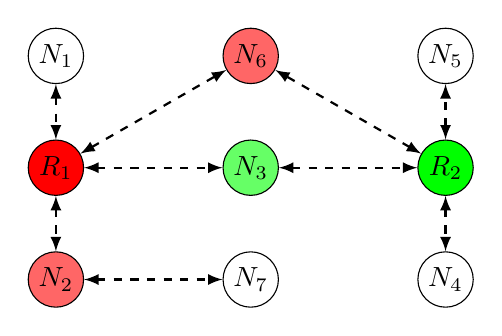
\begin{tikzpicture}[ 
    >=stealth',node distance=3cm, 
    node/.style={circle,minimum size=2.0em,draw}] 
    \node[label=center:$N_1$,node] (N1) [] {}; 
    \node[label=center:$R_1$,node,fill=red] (R1) [below=2em of N1] {}; 
    \node[label=center:$N_2$,node,fill=red!60] (N2) [below=2em of R1] {}; 
    \node[label=center:$N_3$,node,fill=green!60] (N3) [right=5em of R1] {}; 
    \node[label=center:$R_2$,node,fill=green] (R2) [right=5em of N3] {}; 
    \node[label=center:$N_4$,node] (N4) [below=2em of R2] {};
    \node[label=center:$N_5$,node] (N5) [above=2em of R2] {};
    \node[label=center:$N_6$,node,fill=red!60] (N6) [above=2em of N3] {};
    \node[label=center:$N_7$,node] (N7) [below=2em of N3] {};

    \draw[>=latex,auto=right,style={<->},thick,dashed] (N1) -- (R1);
    \draw[>=latex,auto=right,style={<->},thick,dashed] (R1) -- (N2);
    \draw[>=latex,auto=right,style={<->},thick,dashed] (R1) -- (N3);
    \draw[>=latex,auto=right,style={<->},thick,dashed] (N3) -- (R2);
    \draw[>=latex,auto=right,style={<->},thick,dashed] (R2) -- (N4);
    \draw[>=latex,auto=right,style={<->},thick,dashed] (R2) -- (N5);
    \draw[>=latex,auto=right,style={<->},thick,dashed] (R1) -- (N6);
    \draw[>=latex,auto=right,style={<->},thick,dashed] (R2) -- (N6);
    \draw[>=latex,auto=right,style={<->},thick,dashed] (N2) -- (N7);
  \end{tikzpicture}
  \end{center}
  MPRSet($R_1$) = \{$N_2,N_6$\}\newline
  MPRSet($R_2$) = \{$N_3$\}
\end{frame}

\begin{frame}{\insertsubsection}
  \begin{center}
  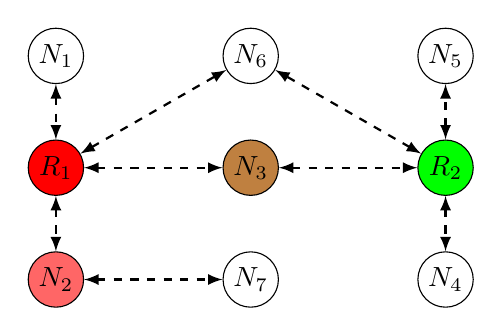
\begin{tikzpicture}[ 
    >=stealth',node distance=3cm, 
    node/.style={circle,minimum size=2.0em,draw}] 
    \node[label=center:$N_1$,node] (N1) [] {}; 
    \node[label=center:$R_1$,node,fill=red] (R1) [below=2em of N1] {}; 
    \node[label=center:$N_2$,node,fill=red!60] (N2) [below=2em of R1] {}; 
    \node[label=center:$N_3$,node,fill=brown] (N3) [right=5em of R1] {}; 
    \node[label=center:$R_2$,node,fill=green] (R2) [right=5em of N3] {}; 
    \node[label=center:$N_4$,node] (N4) [below=2em of R2] {};
    \node[label=center:$N_5$,node] (N5) [above=2em of R2] {};
    \node[label=center:$N_6$,node] (N6) [above=2em of N3] {};
    \node[label=center:$N_7$,node] (N7) [below=2em of N3] {};

    \draw[>=latex,auto=right,style={<->},thick,dashed] (N1) -- (R1);
    \draw[>=latex,auto=right,style={<->},thick,dashed] (R1) -- (N2);
    \draw[>=latex,auto=right,style={<->},thick,dashed] (R1) -- (N3);
    \draw[>=latex,auto=right,style={<->},thick,dashed] (N3) -- (R2);
    \draw[>=latex,auto=right,style={<->},thick,dashed] (R2) -- (N4);
    \draw[>=latex,auto=right,style={<->},thick,dashed] (R2) -- (N5);
    \draw[>=latex,auto=right,style={<->},thick,dashed] (R1) -- (N6);
    \draw[>=latex,auto=right,style={<->},thick,dashed] (R2) -- (N6);
    \draw[>=latex,auto=right,style={<->},thick,dashed] (N2) -- (N7);
  \end{tikzpicture}
  \end{center}
  MPRSet($R_1$) = \{$N_2,N_3$\}\newline
  MPRSet($R_2$) = \{$N_3$\}
\end{frame}

\subsection{WIL($N_3$) > WIL($N_6$)}

\begin{frame}{\insertsubsection}
  \begin{center}
  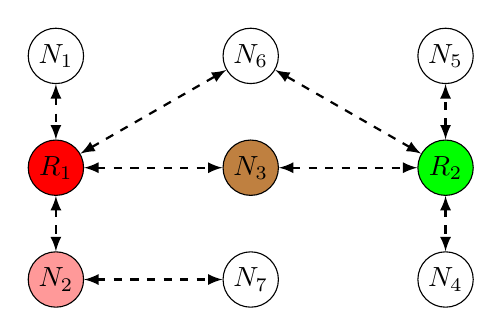
\begin{tikzpicture}[ 
    >=stealth',node distance=3cm, 
    node/.style={circle,minimum size=2.0em,draw}] 
    \node[label=center:$N_1$,node] (N1) [] {}; 
    \node[label=center:$R_1$,node,fill=red] (R1) [below=2em of N1] {}; 
    \node[label=center:$N_2$,node,fill=red!40] (N2) [below=2em of R1] {}; 
    \node[label=center:$N_3$,node,fill=brown] (N3) [right=5em of R1] {}; 
    \node[label=center:$R_2$,node,fill=green] (R2) [right=5em of N3] {}; 
    \node[label=center:$N_4$,node] (N4) [below=2em of R2] {};
    \node[label=center:$N_5$,node] (N5) [above=2em of R2] {};
    \node[label=center:$N_6$,node] (N6) [above=2em of N3] {};
    \node[label=center:$N_7$,node] (N7) [below=2em of N3] {};

    \draw[>=latex,auto=right,style={<->},thick,dashed] (N1) -- (R1);
    \draw[>=latex,auto=right,style={<->},thick,dashed] (R1) -- (N2);
    \draw[>=latex,auto=right,style={<->},thick,dashed] (R1) -- (N3);
    \draw[>=latex,auto=right,style={<->},thick,dashed] (N3) -- (R2);
    \draw[>=latex,auto=right,style={<->},thick,dashed] (R2) -- (N4);
    \draw[>=latex,auto=right,style={<->},thick,dashed] (R2) -- (N5);
    \draw[>=latex,auto=right,style={<->},thick,dashed] (R1) -- (N6);
    \draw[>=latex,auto=right,style={<->},thick,dashed] (R2) -- (N6);
    \draw[>=latex,auto=right,style={<->},thick,dashed] (N2) -- (N7);
  \end{tikzpicture}
  \end{center}
  MPRSet($R_1$) = \{$N_2,N_3$\}\newline
  MPRSet($R_2$) = \{$N_3$\}
\end{frame}

\subsection{WIL($N_3$) < WIL($N_6$)}

\begin{frame}{\insertsubsection}
  \begin{center}
  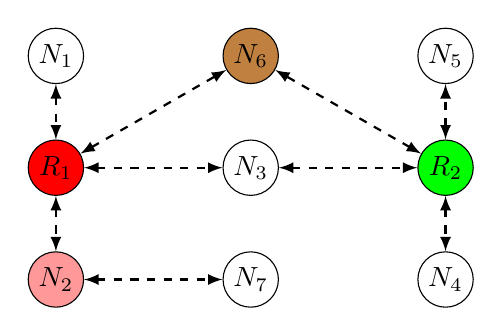
\begin{tikzpicture}[ 
    >=stealth',node distance=3cm, 
    node/.style={circle,minimum size=2.0em,draw}] 
    \node[label=center:$N_1$,node] (N1) [] {}; 
    \node[label=center:$R_1$,node,fill=red] (R1) [below=2em of N1] {}; 
    \node[label=center:$N_2$,node,fill=red!40] (N2) [below=2em of R1] {}; 
    \node[label=center:$N_3$,node] (N3) [right=5em of R1] {}; 
    \node[label=center:$R_2$,node,fill=green] (R2) [right=5em of N3] {}; 
    \node[label=center:$N_4$,node] (N4) [below=2em of R2] {};
    \node[label=center:$N_5$,node] (N5) [above=2em of R2] {};
    \node[label=center:$N_6$,node,fill=brown] (N6) [above=2em of N3] {};
    \node[label=center:$N_7$,node] (N7) [below=2em of N3] {};

    \draw[>=latex,auto=right,style={<->},thick,dashed] (N1) -- (R1);
    \draw[>=latex,auto=right,style={<->},thick,dashed] (R1) -- (N2);
    \draw[>=latex,auto=right,style={<->},thick,dashed] (R1) -- (N3);
    \draw[>=latex,auto=right,style={<->},thick,dashed] (N3) -- (R2);
    \draw[>=latex,auto=right,style={<->},thick,dashed] (R2) -- (N4);
    \draw[>=latex,auto=right,style={<->},thick,dashed] (R2) -- (N5);
    \draw[>=latex,auto=right,style={<->},thick,dashed] (R1) -- (N6);
    \draw[>=latex,auto=right,style={<->},thick,dashed] (R2) -- (N6);
    \draw[>=latex,auto=right,style={<->},thick,dashed] (N2) -- (N7);
  \end{tikzpicture}
  \end{center}
  MPRSet($R_1$) = \{$N_2,N_6$\}\newline
  MPRSet($R_2$) = \{$N_6$\}
\end{frame}

\normalsize
\note[itemize]{
\item Ablauf erklären\newline
\item Willingness ist wichtig für die Wahl des MPRSets\newline
\item MPRs sind i.d.R. auch die Router, wichtige Erkenntnis\newline
\item Weiterleiten der OLSR Messages von R1 nur durch MPR(R1), usw. im letzten Beispiel verwirft N3\newline
\item Funktioniert immer, Beweis über VortexCover (Knoten in einer gültigen Lösung haben max. Abstand 2)\newline
\item Regelmäßige Neuberechnung durch Timeouts und Messages
}

%%% Teil 3 - Problembeschreibung %%%

\section{Wo ist das Problem}

\subsection{Wo ist das Problem}

\begin{frame}{\insertsubsection}
\begin{itemize}
\item Extrem viele Protokolle\newline
\item Viele für AdHoc-Netze\newline
\item Einige energieoptimiert\newline
\item Eines berücksichtigt Art der Stromversorgung\newline
\item Routing nach Ladezustand - Fehlanzeige
\end{itemize}
\end{frame}

\note[itemize]{
\item Bla\newline
\item Bla\newline
\item Also wenig Overhead\newline
\item Ob Energievorrat endlich ist, also Netz oder Batterie\newline
\item Nichts gefunden, vor allem nichts kompatibles!
}

\subsection{Warum wichtig}

\begin{frame}{\insertsubsection}
\begin{itemize}
\item Steigender Bedarf nach Bandbreite und Verfügbarkeit\newline
\item Viele mobile Geräte\newline
\item ABER: Routing braucht Strom\newline
\item Akkuladung begrenzt\newline
\item Routingverfahren berücksichtigen es nicht
\end{itemize}
\end{frame}

\note[itemize]{
\item Wird langfristig mit den zentral arbeitenden Systemen (Funkmast) unnötig aufwändig\newline
\item Nahezu jeder hat ein Smartphone in der Tasche, dass als Router dienen könnte -> Public MESH wird möglich\newline
\item Bla\newline
\item Bla\newline
\item Die Last muss verteilt werden um die Akzeptanz zu steigern -> Lastverteilung nach Akkustand!
}

%%% Teil 4 - Omnet %%%

\section{Omnet}

\subsection{Ganz kurz: Omnet}

\begin{frame}{\insertsubsection}
\begin{itemize}
\item Freie Software, C++, nette Community\newline
\item Ereignisbasiert, Modular\newline
\item Framework INET kann alles, wirklich alles, also viel\newline
\item Inetmanet gibt MANET (AODV okay/buggy, OLSR korrekt)\newline
\item Unbrauchbar: Auswertung -> PERL/Gnuplot (R Versionskonflikte)
\end{itemize}
\end{frame}

\note[itemize]{
\item Keine Warum willst du das-Fragen, einfach Antworten\newline
\item Alles austauschbar, gute Struktur, relativ niedrige Einstiegsschmerzen\newline
\item Von PAN bis Geostationär (manchmal buggy)\newline
\item Fork\newline
\item Kleine Datenmengen teils unterschiedliche Ergebnisse, große Datenmengen lahm/instabil, bestimmte Funktionen gar nicht verfügbar\newline
\item richtig, richtig cooles Spielzeug
}

%%% Teil 5 - Omnet %%%

\section{Simulation}

\subsection{AODV Vanilla}

\begin{frame}{\insertsubsection}
\begin{itemize}
\item Video AODV INIT und FAST
\end{itemize}
\end{frame}

\begin{frame}{\insertsubsection}
\includegraphics[scale=0.45]{aodv-captime}
\end{frame}

\note[itemize]{
\item Man sieht, wie es beginnt und wie der Akku nach und nach geleert wird, erst dann Umschaltung\newline
\item Nur senden verbraucht Strom (besser erkennbar, Rest in der Natur nicht beeinflussbar)\newline
\item OLSR zeigt selbes Verhalten\newline
\item AODV Implementation manchmal instabil (Vanilla), scheinbar nicht 100\% korrekt implementiert, Instabilität durch feste Seeds umgangen
}

\begin{frame}{\insertsubsection}
  \begin{center}
\includegraphics[scale=0.45]{aodv-100}
  \end{center}
\end{frame}

\note[itemize]{
\item 100 Simulationen mit verschiedenen Zufallszahlen\newline
\item Ergebnisse sehr stabil
}

\subsection{Da geht doch was ...}

\begin{frame}{\insertsubsection}
  \begin{center}
\includegraphics[scale=0.4]{kid1}
  \end{center}
\end{frame}

\subsection{Ziele}

\begin{frame}{\insertsubsection}
\begin{itemize}
\item Lastverteilung nach relativem Akkustand\newline
\item Kompatibilität zu anderen Systemen\newline
\item Steuerung der Empfindlichkeit und Grad der Anpassung\newline
\end{itemize}
\end{frame}

\note[itemize]{
\item Bla\newline
\item Gemischte Netze sollen funktionieren\newline
\item Parameter um die ladungsabhängige Anpassung zu steuern
}

\subsection{Ideen}

\begin{frame}{\insertsubsection}
\begin{itemize}
\item Es muss ein vorhandener Parameter eingesetzt werden\newline
\item AODV: HopCount künstlich anheben (begrenzt möglich)\newline
\item OLSR: Willingness ändern
\end{itemize}
\end{frame}

\note[itemize]{
\item Im Prinzip sollen sich die Router schlechter machen, als sie sind, gerade in der heutigen Zeit eher selten zu beobachten \newline
\item Begrenzt durch maximalen HopCount (8Bit = 255) - größeres Netz, schwächere Anhebung\newline
\item Prinzipiell keine Grenze in der Größe des Netzes gesetzt. Dafür weniger fein steuerbar
}

\subsection{Mit Mathe muss man rechnen...}

\begin{frame}{\insertsubsection}
  \begin{center}
\includegraphics[scale=0.75]{kid2}
  \end{center}
\end{frame}

\subsection{AODVPO}

\begin{frame}{\insertsubsection}
\begin{itemize}
\item Drei Parameter\newline
\begin{itemize}
\item Trigger $t \in \interval{0.1}{0.9}$ \newline
\item Sensitivity $s \in \mathbb{R^{+}}$\newline
\item Bias $B \in \mathbb{N}_0$\newline
\end{itemize}
\item Ein Ziel\newline
\begin{itemize}
\item HopCount $H_{neu} = H_{alt} + 1 \rightarrow H'_{neu} = H_{alt} + 1 + P$ \newline
\item wobei Penalty $P = \lceil\frac{s}{C(i)} + B\rceil$\newline
\end{itemize}
\end{itemize}
\end{frame}

\begin{frame}{\insertsubsection}
\begin{itemize}
\item Trigger $t = 0.2$ bedeutet, dass bei $C(i) \in \{0.8,0.6,...,0.2\}$ eine Anpassung stattfinden soll\newline
\item Allgemeiner: Es wird eine Anpassung ausgelöst, wenn gilt: \newline $(C(i) * 100) \mod(100t) = 0$\newline
\item $C(i) \in \interval[open left]{0}{1}$ entspricht dem relativen Ladezustand\newline
\item Anpassung meint das Versenden von RERR, dadurch Ausfall und Neuberechnung
\end{itemize}
\end{frame}

\note[itemize]{
\item Hoher Trigger bringt schnellere Reaktion, dafür mehr Ausfall (Paketverlust)
}

\begin{frame}{\insertsubsection}
\begin{itemize}
\item Penalty $P(s,C(i),B) = \lceil\frac{s}{C(i)} + B\rceil$ ist der Wert, der auf den neuen Hopcount $H'_{neu}$ aufgeschlagen wird\newline
\item $P(2,0.6,0) = \lceil\frac{2}{0.6} + 0\rceil = 4$\newline
\item $H'_{neu} = H_{alt} + 1 + 4 > H_{neu} = H_{alt} + 1$\newline
\item Nulldivision unmöglich (Akku leer!)
\end{itemize}
\end{frame}

\begin{frame}{\insertsubsection}
\begin{itemize}
\item Implementierung relativ einfach\newline
\item Funktioniert nicht bzw. zufällig\newline
\item Diagnose: AODV fehlerhaft\newline
\item Therapie: Wartezeit $W(P)$ bevor RREP erzeugt wird
\end{itemize}
\end{frame}

\note[itemize]{
\item 3 Methoden erstellen, Einfügen in Hopberechnung an mehreren Stellen \newline
\item Warum nicht? Logs passen...\newline
\item Wertet nicht den HC aus, sondern nimmt erstes empfangenes RREP ... macht aber begrenzt Sinn ... \newline
\item Dann funktioniert es ... meistens ... weitergehendes Reparieren von AODV außerhalb des Umfangs dieser Arbeit ... gute paar tausend Zeilen Code 
}

\subsection{AODVPO Live}

\begin{frame}{\insertsubsection}
\begin{itemize}
\item Video AODVPO FAST, RENEG
\end{itemize}
\end{frame}

\begin{frame}{\insertsubsection}
\includegraphics[scale=0.45]{aodvpo-captime}
\end{frame}

\begin{frame}{\insertsubsection}
\includegraphics[scale=0.45]{aodvpohappy-captime}
\end{frame}

\begin{frame}{\insertsubsection}
\includegraphics[scale=0.45]{aodvposloppy-captime}
\end{frame}

\begin{frame}{\insertsubsection}
\includegraphics[scale=0.45]{aodvpo-captime-bad}
\end{frame}

\begin{frame}{\insertsubsection}
\includegraphics[scale=0.45]{aodvpo-100}
\end{frame}

\note[itemize]{
\item Größere Streuung durch Zufall und Fehlfunktion\newline
\item Alter Wert ca 0,4, immer besser!!!\newline
\item Wie sehen dann eigentlich optimale Parameter aus?\newline
}

\subsection{Studies}

\begin{frame}{\insertsubsection}
\includegraphics[scale=0.45]{aodvstudycap}
\end{frame}

\note[itemize]{
\item Äußerst zufrieden, schaute mir mal die Simulation mit Abweichung fast Null an\newline
\item s zwischen 0.5 und 5, t zwischen 0.1 und 0.9 laufen lassen - macht man t kleiner oder s größer kommen sehr extreme werte raus
\item Erkannte ein weiteres Problem: Es wurde nur ein gewissen Prozentsatz an Paketen erfolgreich übertragen, nämlich:
}

\begin{frame}{\insertsubsection}
\begin{center}
\Huge{0}
\normalsize
... ist auch ein Prozentsatz
\end{center}
\end{frame}

\note[itemize]{
\item Ursachen: Kein Zustandkommen von Routen durch ständige RERR oder zu hohem HopCount (oder intabiles Verhalten bei Pufferüberlauf HopCount 8Bit) oder Simpel Fehlfunktion Protokoll AODV
}

\begin{frame}{\insertsubsection}
\includegraphics[scale=0.45]{aodvstudyudp}
\end{frame}

\note[itemize]{
\item Um jetzt einen sinnvollen Zusammenhang zu finden, muss man das kombienieren. Prinzip: Ein hoher Loss oder Abweichung disqualifiziert das Setting
}

\subsection{Performance}

\begin{frame}{\insertsubsection}
\begin{itemize}
\item Performance $F = ( 1 - ( L + c ) ) / ( M + c )$\newline
\item Standardabweichung der Ladestände $M = \sqrt{\sum_{i=1}^{n} \frac{(C(i)-\bar{x})^2}{n}}$
\begin{itemize}
\item Sei $n$ die Anzahl der Router,
\item $C(i)$ die Restladung des jeweiligen Routers $i$ und 
\item $\bar{x} = \sum_{i=1}^{n} \frac{C(i)}{n}$ das arithmetische Mittel der Restladungen\newline
\end{itemize}
\item $L$ ist der durchschnittliche PaketLoss aller Übertragungen\newline
\item $c = 10^{-10}$ (kontant)
\end{itemize}
\end{frame}

\begin{frame}{\insertsubsection}
\includegraphics[scale=0.45]{aodvstudyperf}
\end{frame}

\begin{frame}{\insertsubsection}
\includegraphics[scale=0.45]{aodvstudyperfmap}
\end{frame}

\note[itemize]{
\item Das brachte t = 0,2 und s = 3 für die o.g. Ergebnisse
}
\subsection{OLSR}

\begin{frame}{\insertsubsection}
\begin{itemize}
\item Prinzipiell stabiler\newline
\item Statt HopCount-Penalty neue Willingness $W_{neu} = \lfloor\max(1,(7\cdot C(i)\cdot (1-s)-B))\rfloor$ berechnet\newline
\item Fließender Übergang\newline
\item Keine Hacks
\end{itemize}
\end{frame}

\note[itemize]{
\item Sauberer implementiert in Vanilla, weniger Ausreißer
\item keine Extremen Werte, dafür nicht so genau im Zeitpunkt, dafür keine Unterbrechungen
\item Man kann in diesem Szenario (bei OLSR läuft akku leer) sogar den Overhead senken, da man die Intervalle größer machen kann in denen Kontrollnachrichten geschickt werden
}

\subsection{Vergleich}


\begin{frame}{\insertsubsection}
\includegraphics[scale=0.35]{compare-capdev}
\end{frame}

\begin{frame}{\insertsubsection}
\includegraphics[scale=0.35]{compare-capdev-short}
\end{frame}

\begin{frame}{\insertsubsection}
\includegraphics[scale=0.35]{compoverhead}
\end{frame}

\note[itemize]{
\item Intervalle bei OLSRPO verdoppelt was den Stromverbrauch reduziert, trotzdem bessere Werte
}

\begin{frame}{\insertsubsection}
\includegraphics[scale=0.35]{packetloss}
\end{frame}

\note[itemize]{
\item OLSR Vanilla und AODVPO Trigger Happy entfernt, da zu extreme Werte das Bild verzerren bzw. die anderen Werte unlesbar machen
}

\section{Abschluss}

\subsection{Fazit}

\begin{frame}{\insertsubsection}
\begin{itemize}
\item Funktioniert in den gezeigten Szenarien\newline 
\item Funktioniert in gemischten Netzen (Kompatibel)\newline 
\item Funktioniert in größeren Netzen (Skaliert)\newline 
\end{itemize}
\end{frame}

\note[itemize]{
\item Haben wir gesehen\newline
\item Nicht so gut, aber grundsätzlich funktioniert es, bei OLSR besser als bei AODV, was vielleicht wieder an der Implementierung liegt\newline
\item dito
}

%\subsection{Und sonst?}
%
%\begin{frame}{\insertsubsection}
%\begin{itemize}
%\item Andere Parameter denkbar, wie CPU Last, verfügbare Bandbreite, ...\newline
%\item Implementierung von OLSRPO auf Android und Test?\newline
%\end{itemize}
%\end{frame}

%%% Ende %%%

\section*{Ende} 

%\begin{frame}{Thanks for the fish and goodbye!}
%\includegraphics[scale=0.160]{folks} \newline
%\tiny{Quelle: http://outlawjimmy.com/wp-content/uploads/2013/04/thatsallfolks.jpg}
%\end{frame}

\begin{frame}{Das wars! Fragen?}
  \includemedia[
    width=0.8\linewidth,height=0.6\linewidth,
    activate=pageopen,
    addresource=neindochoh.flv,        %adjust
    flashvars={source=neindochoh.flv}  %adjust
  ]{\frame{\includegraphics[scale=0.45]{neindochoh}}}{VPlayer9.swf}

%\movie[
%  height = 6cm,
%  width = 8cm,
%  showcontrols=true,
%  autostart=true,
%  poster
%] 
%{}{neindochoh.mpg}

\end{frame}



\subsection{Möchten Sie mehr wissen?}

\begin{frame}{\insertsubsection}
\begin{itemize}
\item RFC 3626 OLSR
\item RFC 3561 AODV, Draft 01 IPv6
\item Nitin Kumar, Parvez Ahmed Alvi, Ajay Singh Yadav, and Anupam Swami.
A study of routing protocols for ad-hoc network. International Journal of Application or Innovation in Engineering and Management, 2(6):154–159, Juni 2013.
\item Stefano Basagni, Marco Conti, Silvia Giordano, and Ivan Stojmenovic. IEEE
802.11 AD HOC Networks: Protocols, Performance, and Open Issues, page
416ff. WileyIEEE Press, Piscataway, NJ, USA, 2004.
\item DIY: https://github.com/marcelebbrecht/powerrouting
\end{itemize}
\end{frame}

\end{document}